\documentclass[12pt,a4paper]{article}

% ─── Page Layout ───────────────────────────────────────────────────────────────
\usepackage[a4paper, margin=0.8in, headheight=14pt]{geometry}

% ─── Fonts (XeLaTeX) ───────────────────────────────────────────────────────────
\usepackage{fontspec}
\usepackage{unicode-math}
\setmainfont{TeX Gyre Pagella}
\setmonofont[Scale=0.88]{TeX Gyre Cursor}
\setmathfont{Latin Modern Math}

% ─── Packages ──────────────────────────────────────────────────────────────────
\usepackage{xcolor}
\usepackage{colortbl}
\usepackage{titlesec}
\usepackage{enumitem}
\usepackage{tabularx}
\usepackage{booktabs}
\usepackage{array}
\usepackage{amsmath}
\usepackage{tikz}
\usetikzlibrary{shapes.geometric, arrows.meta, positioning, calc, fit, decorations.pathreplacing, patterns}
\usepackage{tcolorbox}
\tcbuselibrary{skins, breakable}
\usepackage{hyperref}
\usepackage{fancyhdr}
\usepackage{graphicx}
\usepackage{microtype}
\hyphenpenalty=10000
\exhyphenpenalty=10000
\sloppy
\usepackage{caption}
\usepackage{setspace}
\usepackage{multirow}
\usepackage{tocloft}

% ─── Q&A helper ────────────────────────────────────────────────────────────────
\newcommand{\Q}[1]{\textbf{#1}\par\noindent\ignorespaces}

% ─── Colour Palette ────────────────────────────────────────────────────────────
\definecolor{myred}{RGB}{196,30,58}
\definecolor{mydark}{RGB}{30,30,50}
\definecolor{mygreen}{RGB}{14,120,80}
\definecolor{myteal}{RGB}{0,130,140}
\definecolor{myamber}{RGB}{180,100,0}
\definecolor{mypurple}{RGB}{100,30,160}
\definecolor{mygray}{RGB}{246,247,249}
\definecolor{mgframe}{RGB}{180,185,200}
\definecolor{watermark}{RGB}{145,150,170}
\definecolor{hdrred}{RGB}{250,232,235}
\definecolor{hdrgreen}{RGB}{220,244,233}
\definecolor{hdrteal}{RGB}{220,242,244}
\definecolor{hdramber}{RGB}{253,242,215}
\definecolor{hdrpurple}{RGB}{238,228,255}
\definecolor{hdrgray}{RGB}{238,240,245}
\definecolor{rowalt}{RGB}{250,251,253}

% ─── Section Formatting ────────────────────────────────────────────────────────
\titleformat{\section}
  {\large\bfseries\color{myred}}{\thesection.}{0.5em}{}
  [\vspace{1pt}{\color{myred}\rule{\linewidth}{0.8pt}}]
\titleformat{\subsection}
  {\normalsize\bfseries\color{myteal}}{\thesubsection}{0.5em}{}
\titlespacing*{\section}{0pt}{18pt}{7pt}
\titlespacing*{\subsection}{0pt}{11pt}{4pt}

% ─── Paragraph ─────────────────────────────────────────────────────────────────
\setlength{\parindent}{0pt}
\setlength{\parskip}{4pt}

% ─── TOC Styling ───────────────────────────────────────────────────────────────
\renewcommand{\cfttoctitlefont}{\large\bfseries\color{myred}}
\renewcommand{\cftaftertoctitle}{\par\noindent{\color{myred}\rule{\linewidth}{0.8pt}}}
\setlength{\cftbeforetoctitleskip}{0pt}
\setlength{\cftaftertoctitleskip}{6pt}
\renewcommand{\cftsecfont}{\normalsize\bfseries\color{mydark}}
\renewcommand{\cftsecpagefont}{\normalsize\bfseries\color{mydark}}
\renewcommand{\cftsecleader}{\cftdotfill{\cftdotsep}}
\setlength{\cftbeforesecskip}{7pt}
\renewcommand{\cftsubsecfont}{\small\color{mydark}}
\renewcommand{\cftsubsecpagefont}{\small\color{mydark}}
\setlength{\cftbeforesubsecskip}{3pt}
\setlength{\cftsubsecindent}{1.4em}

% ─── Table helpers ─────────────────────────────────────────────────────────────
\renewcommand{\arraystretch}{1.45}
\setlength{\tabcolsep}{6pt}
\arrayrulecolor{mydark}
\newcolumntype{B}[1]{>{\small\bfseries\raggedright\arraybackslash}m{#1}}
\newcolumntype{Y}{>{\small\raggedright\arraybackslash}X}
\renewcommand{\tabularxcolumn}[1]{m{#1}}

% ─── Header / Footer ───────────────────────────────────────────────────────────
\pagestyle{fancy}
\fancyhf{}
\fancyhead[L]{\small\color{myred}\textbf{EC403}\;\color{mydark}--- Microprocessor and Microcontroller}
\fancyhead[R]{\small\color{myteal}\textbf{Module 3 Notes}}
\fancyfoot[C]{\small\color{mydark}\thepage}
\fancyfoot[R]{\small\color{watermark}\textit{\copyright\ Biraj}}
\renewcommand{\headrulewidth}{0.5pt}
\renewcommand{\footrulewidth}{0.3pt}

% ─── Hyperref ──────────────────────────────────────────────────────────────────
\hypersetup{
  colorlinks=true, linkcolor=myteal, urlcolor=myteal,
  pdfauthor={Biraj Sarkar (CGEC)},
  pdftitle={EC403 --- Module 3 Notes: Virtual Memory, Cache, x86 Evolution and 8051}
}

% ─── tcolorbox styles ──────────────────────────────────────────────────────────
\tcbset{
  tikzbox/.style={
    colback=mygray, colframe=mgframe, boxrule=0.6pt, arc=4pt,
    left=8pt, right=8pt, top=6pt, bottom=6pt,
    colbacktitle=mgframe, coltitle=mydark, fonttitle=\small\bfseries
  },
  defbox/.style={
    colback=hdrgreen, colframe=mygreen, boxrule=0.8pt, arc=4pt,
    left=9pt, right=9pt, top=6pt, bottom=6pt,
    colbacktitle=mygreen, coltitle=white, fonttitle=\small\bfseries
  },
  formulabox/.style={
    colback=hdrteal, colframe=myteal, boxrule=0.8pt, arc=4pt,
    left=9pt, right=9pt, top=7pt, bottom=7pt,
    colbacktitle=myteal, coltitle=white, fonttitle=\small\bfseries
  },
  examplebox/.style={
    colback=hdramber, colframe=myamber, boxrule=0.8pt, arc=4pt,
    left=9pt, right=9pt, top=6pt, bottom=6pt,
    colbacktitle=myamber, coltitle=white, fonttitle=\small\bfseries
  },
  masonbox/.style={
    colback=hdrpurple, colframe=mypurple, boxrule=0.8pt, arc=4pt,
    left=9pt, right=9pt, top=6pt, bottom=6pt,
    colbacktitle=mypurple, coltitle=white, fonttitle=\small\bfseries
  },
  exambox/.style={
    colback=hdrpurple, colframe=mypurple, boxrule=1pt, arc=5pt,
    left=10pt, right=10pt, top=8pt, bottom=8pt,
    colbacktitle=mypurple, coltitle=white, fonttitle=\bfseries,
    breakable, title after break={\textbf{Frequently Asked / Viva Questions (contd.)}}
  }
}
\tcbset{breakable}
\tcbset{after={\par\color{black}}}

% ─── TikZ styles ───────────────────────────────────────────────────────────────
\tikzset{
  block/.style={rectangle, draw=myteal, fill=hdrteal,
    text width=2.4cm, align=center, minimum height=0.95cm,
    font=\small, rounded corners=3pt, line width=0.7pt},
  redblock/.style={rectangle, draw=myred, fill=hdrred,
    text width=2.4cm, align=center, minimum height=0.95cm,
    font=\small, rounded corners=3pt, line width=0.7pt},
  sumjunc/.style={circle, draw=myamber, fill=hdramber,
    minimum size=0.62cm, font=\small, line width=0.8pt},
  arrow/.style={-Stealth, thick, color=mydark},
  redarrow/.style={-Stealth, thick, color=myred},
  line/.style={thick, color=mydark}
}

\begin{document}

% ─── Title Page ───────────────────────────────────────────────────────────────
\begin{center}
  {\LARGE\bfseries\color{myred} EC403 --- Microprocessor and Microcontroller}\\[5pt]
  {\normalsize\color{mydark} Semester IV \quad$\bullet$\quad 3L:0T:0P \quad$\bullet$\quad 3 Credits}\\[3pt]
  {\normalsize\color{myteal}\textbf{Module 3 Exam Notes: Virtual Memory, Cache, x86 Evolution and 8051}}\\[3pt]
  {\small\color{mydark} CGEC \;$|$\; B.Tech ECE (2023--27) \;$|$\; \textit{Biraj Sarkar}}
\end{center}
\vspace{2pt}
\noindent{\color{myred}\rule{\linewidth}{1.5pt}}
\vspace{2pt}

\hypersetup{linkcolor=mydark}
\tableofcontents
\hypersetup{linkcolor=myteal}
\newpage

\section{Memory Hierarchy, x86 Evolution and 8051}
\subsection{Virtual Address Space and Paging}
\begin{tcolorbox}[defbox,title={Virtual Address Space}]
\textbf{Virtual memory} gives each process its own view of memory. The processor generates a virtual address, which the memory management unit (MMU) translates to a physical address. Translation allows isolation, controlled sharing and keeping only the currently needed parts of an address space in RAM.
\end{tcolorbox}
\par\addvspace{7pt}\noindent
A \textbf{page} is a fixed-size virtual block. A \textbf{frame} is an equally sized physical block. A page-table entry identifies the frame when present and records access permissions. Hardware may also track whether a page was accessed or written. The page offset is the position within a page and is unchanged by translation.
\begin{tcolorbox}[tikzbox,title={Paged Address Translation}]
\centering
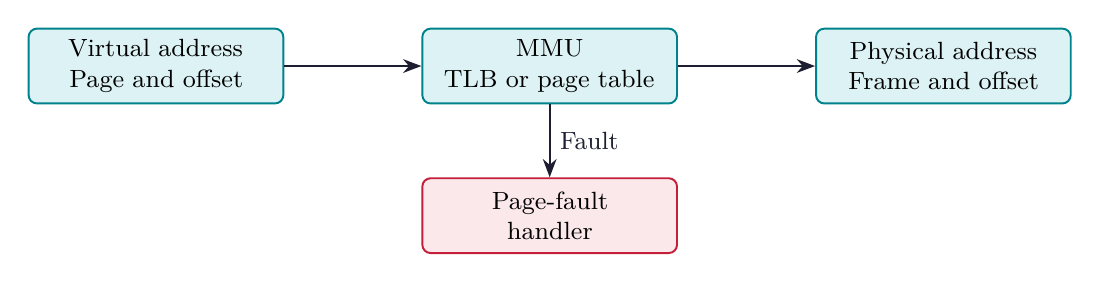
\begin{tikzpicture}
\node[block,text width=3cm] (v) at (0,0) {Virtual address\\Page and offset};
\node[block,text width=3cm] (m) at (5,0) {MMU\\TLB or page table};
\node[block,text width=3cm] (p) at (10,0) {Physical address\\Frame and offset};
\draw[arrow] (v) -- (m);
\draw[arrow] (m) -- (p);
\node[redblock,text width=3cm] (f) at (5,-1.9) {Page-fault\\handler};
\draw[arrow] (m) -- (f) node[midway,right,font=\small] {Fault};
\end{tikzpicture}
\end{tcolorbox}
\par\addvspace{7pt}\noindent
The \textbf{translation lookaside buffer (TLB)} caches translations. A TLB hit can avoid a page-table walk. On a TLB miss, hardware or software searches the page table. A present and permitted page can refill the TLB without disk access. A page fault transfers control to the operating system. An invalid access may be rejected. A valid demand-paged access can allocate a frame, evict a victim if needed, write it back if dirty and backed by writable storage, load or create the requested page, update translation state, and restart the instruction.
\begin{tcolorbox}[examplebox,title={Translate a Virtual Address}]
With 4 KiB pages and virtual address \texttt{12345H},
\begin{align*}
 \text{page size} &= 4096=2^{12}\ \text{bytes},\\
 \text{virtual page} &= \text{\texttt{12H}},\qquad
 \text{offset} = \text{\texttt{345H}}.
\end{align*}
If the page maps to frame \texttt{2AH}, the physical address is \texttt{2A000H + 345H = 2A345H}. A TLB miss alone does not imply a page fault.
\end{tcolorbox}
\subsection{Paging, Segmentation and Replacement}
\textbf{Segmentation} uses variable-size logical regions. A selector identifies a descriptor with base, limit and permissions. Adding the offset to the base gives the linear address when checks pass. Segmentation can leave external holes. Paging uses fixed-size frames and can leave unused space in the last page of an allocation. The two mechanisms can coexist.
When no frame is free, FIFO evicts the oldest resident page and least recently used (LRU) favours a page that has not recently been referenced. Clock is an approximation based on an accessed bit. If active pages are repeatedly evicted and needed again, the system can spend much of its time handling faults. This is \textbf{thrashing}.

\section{Cache Memory}
\begin{tcolorbox}[defbox,title={Cache, Hit and Miss}]
A \textbf{cache} holds copies of recently or nearby accessed memory blocks in fast storage. A \textbf{hit} finds the requested block in the cache. A \textbf{miss} fetches it from a lower level. Temporal locality means recently used data is likely to be reused. Spatial locality means nearby data is likely to be accessed soon.
\end{tcolorbox}
\par\addvspace{7pt}\noindent
Each cache line stores a block, a tag and a valid bit. A write-back cache also tracks whether the line is dirty. The address offset selects a byte within a block. The index selects a set, and the tag distinguishes memory blocks that use that set.
\par\addvspace{6pt}
\begingroup
\setlength{\extrarowheight}{2.5pt}
\noindent\begin{tabularx}{\linewidth}{|B{3.5cm}|Y|Y|}
\hline
\textbf{Mapping} & \textbf{Placement} & \textbf{Trade-off} \\ \hline
Direct mapped & One location for each block. & Fast lookup, more conflict misses. \\ \hline
Fully associative & Any line is eligible. & Fewer placement conflicts, more tag comparisons. \\ \hline
Set associative & Any of $W$ lines in one indexed set. & Balances comparison hardware and flexibility. \\ \hline
\end{tabularx}\par
\endgroup
\subsection{Write Policies and Misses}
\textbf{Write-through} updates the lower level when the cache is written, often through a write buffer. \textbf{Write-back} updates the cache and writes dirty blocks to the lower level when required, for example on eviction. \textbf{Write-allocate} fetches a line after a write miss, while \textbf{no-write-allocate} sends that write to the lower level without allocating the line. These are separate design decisions.
First-use misses are compulsory. Capacity misses arise when the cache is too small for the active blocks. Conflict misses arise when multiple blocks compete for the same set. In an associative set, LRU, approximate LRU or another policy chooses the victim if every way is occupied.
\begin{tcolorbox}[examplebox,title={Cache Address Fields and Average Access Time}]
For 32-bit byte addresses, a 16 KiB, four-way cache with 32-byte lines has
\begin{align*}
 \text{sets} &= 16384/(4\cdot32)=128,\\
 \text{offset bits} &= \log_2 32=5,\\
 \text{index bits} &= \log_2 128=7,\\
 \text{tag bits} &=32-5-7=20.
\end{align*}
If the hit time is 2 ns, the miss rate is 5\% and the \emph{additional} miss penalty is 40 ns, the average memory access time is $2+0.05(40)=4$ ns.
\end{tcolorbox}

\begin{tcolorbox}[examplebox,title={Identify Two Blocks That Conflict}]
A direct-mapped cache has eight lines and four bytes per block. For byte address $a$, the memory block number is $\lfloor a/4\rfloor$, and the line index is the block number modulo eight.
\begin{align*}
 a=4 &: \quad \text{block }1,\ \text{line }1,\ \text{tag }0,\\
 a=36 &: \quad \text{block }9,\ \text{line }1,\ \text{tag }1.
\end{align*}
With an empty cache, accesses to $4,36,4$ all miss. The third miss happens because the second access replaced the first block, even though other lines were free. The same blocks could coexist in a two-way set with two available ways.
\end{tcolorbox}

\section{80286, 80486 and Pentium Architectures}
The syllabus groups these under advanced coprocessor architectures. The 80286, 80486 and Pentium are main x86 processors. The comparison tracks how memory management and numeric coprocessor functions evolved.
\subsection{80286 Protected Mode and 80287}
The 80286 has a 16-bit data bus and a 24-bit physical address bus, giving up to 16 MiB of physical memory in protected mode. Real-address mode supports the 8086-style environment. Protected mode uses segment descriptors, access checks and four privilege levels. Selectors locate descriptors in the global or local descriptor table. Descriptors record the segment base, limit and access rights. The 80286 provides segment-based virtual memory support without hardware paging. The optional 80287 performs x87 floating-point operations.
\subsection{80486 Integration}
The original i486DX uses a 32-bit data bus, a 32-bit physical address space and a scalar instruction pipeline. It integrates an 8 KiB unified L1 cache, x87 floating-point unit (FPU), segmentation and hardware paging. A unified cache shares capacity between instructions and data. The 486SX variant does not provide a usable on-chip FPU. These details refer to the original models, since later 486 parts varied.
\subsection{Original Pentium Superscalar Execution}
A \textbf{superscalar} processor can issue more than one instruction in a cycle when the instructions can execute together. The original Pentium uses U and V integer pipelines. The U pipe accepts the broader instruction set, while the V pipe accepts eligible simple instructions in supported pairs. A data dependency or a pairing restriction can prevent dual issue. The processor adds dynamic branch prediction, separate 8 KiB instruction and 8 KiB data L1 caches, integrated floating-point hardware, a 64-bit external data bus and 32-bit physical addressing. The external data bus width is distinct from operand and address width.
\par\addvspace{6pt}
\begingroup
\setlength{\extrarowheight}{2.5pt}
\noindent\begin{tabularx}{\linewidth}{|B{3.0cm}|Y|Y|Y|}
\hline
\textbf{Feature} & \textbf{80286} & \textbf{i486DX} & \textbf{Original Pentium} \\ \hline
External data bus & 16 bits & 32 bits & 64 bits \\ \hline
Physical address bits & 24 & 32 & 32 \\ \hline
Protected memory & Segmentation & Segmentation and paging & Segmentation and paging \\ \hline
On-chip L1 & No & 8 KiB unified & 8 KiB I + 8 KiB D \\ \hline
Numeric unit & Optional 80287 & Integrated x87 & Integrated x87 \\ \hline
\end{tabularx}\par
\endgroup

\section{Classic 8051 System, Pinout and Ports}
\begin{tcolorbox}[defbox,title={Classic 8051 Microcontroller}]
The original Intel 8051 is an 8-bit microcontroller with 4 KiB on-chip program ROM, 128 bytes of internal RAM, 32 I/O lines, two 16-bit timers, a serial port and five interrupt sources. It has separate code and data address spaces. Its accumulator A processes byte data, B assists multiply and divide, PSW contains flags and register-bank selection, DPTR is a 16-bit pointer, and PC and SP control instruction and stack access.
\end{tcolorbox}
\par\addvspace{8pt}
\begin{tcolorbox}[tikzbox,unbreakable,title={Classic 8051 40-Pin DIP, Top View}]
\centering
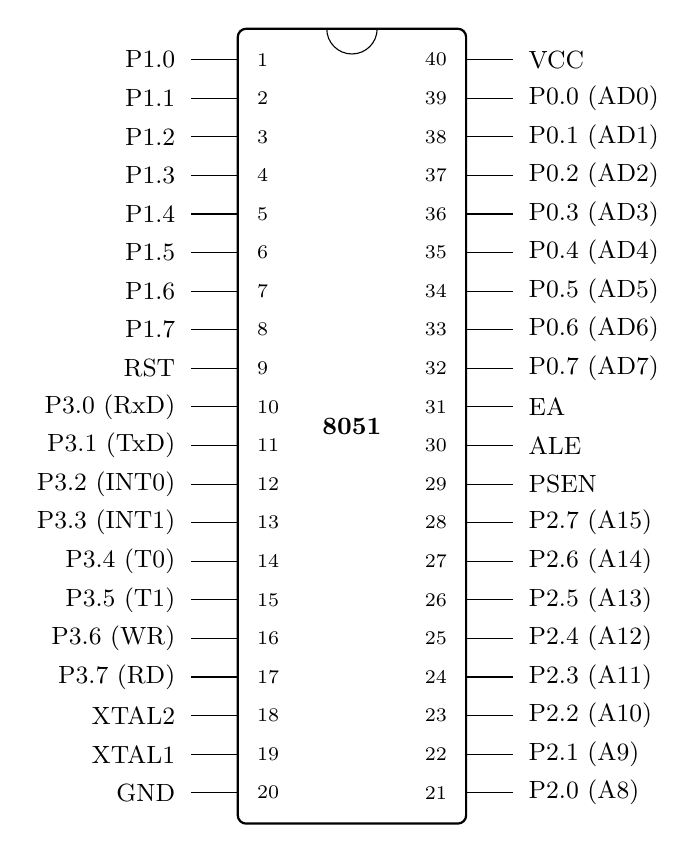
\begin{tikzpicture}[x=1cm,y=0.49cm,every node/.style={font=\small}]
\draw[thick,rounded corners=3pt] (-1.45,0.8) rectangle (1.45,-19.8);
\draw (-0.32,0.8) arc[start angle=180,end angle=360,radius=0.32cm];
\node[font=\small\bfseries] at (0,-9.5) {8051};
\foreach \i/\leftpin/\rightpin in {
0/P1.0/VCC,1/P1.1/P0.0 (AD0),2/P1.2/P0.1 (AD1),3/P1.3/P0.2 (AD2),
4/P1.4/P0.3 (AD3),5/P1.5/P0.4 (AD4),6/P1.6/P0.5 (AD5),7/P1.7/P0.6 (AD6),
8/RST/P0.7 (AD7),9/P3.0 (RxD)/EA,10/P3.1 (TxD)/ALE,11/P3.2 (INT0)/PSEN,
12/P3.3 (INT1)/P2.7 (A15),13/P3.4 (T0)/P2.6 (A14),14/P3.5 (T1)/P2.5 (A13),
15/P3.6 (WR)/P2.4 (A12),16/P3.7 (RD)/P2.3 (A11),17/XTAL2/P2.2 (A10),
18/XTAL1/P2.1 (A9),19/GND/P2.0 (A8)} {
  \pgfmathtruncatemacro{\lp}{\i+1}
  \pgfmathtruncatemacro{\rp}{40-\i}
  \draw (-1.45,-\i) -- (-2.05,-\i) node[left=2pt] {\leftpin};
  \draw (1.45,-\i) -- (2.05,-\i) node[right=2pt] {\rightpin};
  \node[anchor=west,font=\scriptsize] at (-1.33,-\i) {\lp};
  \node[anchor=east,font=\scriptsize] at (1.33,-\i) {\rp};
}
\end{tikzpicture}
\par\vspace{7pt}
EA, PSEN, INT0, INT1, WR and RD are active low. The drawing uses pin names without overbars for readability.
\end{tcolorbox}

\begin{tcolorbox}[tikzbox,title={8051 System Building Blocks}]
\centering
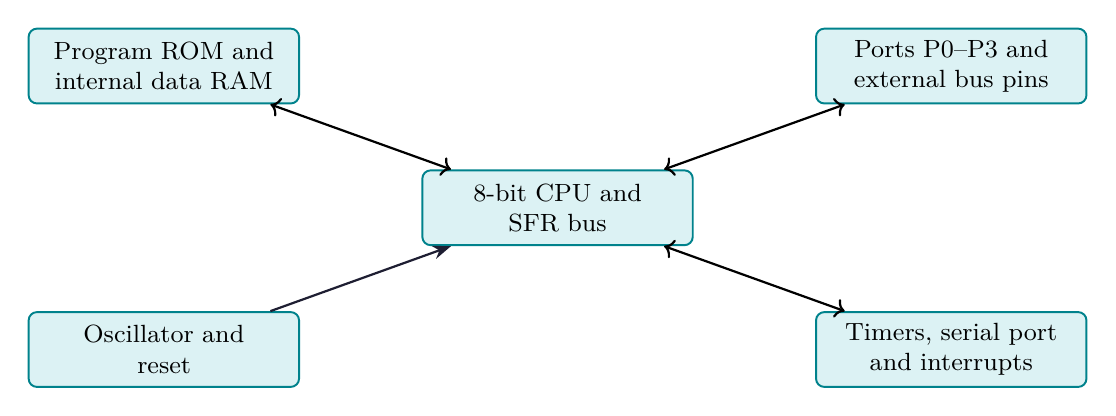
\begin{tikzpicture}
\node[block,text width=3.2cm] (core) at (0,0) {8-bit CPU and\\SFR bus};
\node[block,text width=3.2cm] (mem) at (-5,1.8) {Program ROM and\\internal data RAM};
\node[block,text width=3.2cm] (ports) at (5,1.8) {Ports P0--P3 and\\external bus pins};
\node[block,text width=3.2cm] (clock) at (-5,-1.8) {Oscillator and\\reset};
\node[block,text width=3.2cm] (peri) at (5,-1.8) {Timers, serial port\\and interrupts};
\draw[<->,thick] (core) -- (mem);
\draw[<->,thick] (core) -- (ports);
\draw[arrow] (clock) -- (core);
\draw[<->,thick] (core) -- (peri);
\end{tikzpicture}
\end{tcolorbox}
\subsection{Pin and Port Roles}
\par\addvspace{5pt}
\begingroup
\setlength{\extrarowheight}{2.5pt}
\noindent\begin{tabularx}{\linewidth}{|B{2.6cm}|B{2.4cm}|Y|}
\hline
\textbf{Signals} & \textbf{Pins} & \textbf{Uses and electrical behaviour} \\ \hline
P0 & 32--39 & AD7--AD0 in external bus cycles. In ordinary GPIO use it is open drain, so add pull-ups for a driven high level. \\ \hline
P1 & 1--8 & General-purpose quasi-bidirectional I/O with internal pull-ups on the original 8051. \\ \hline
P2 & 21--28 & GPIO or A8--A15 for external code fetch and 16-bit external-data addressing. \\ \hline
P3 & 10--17 & GPIO with internal pull-ups and eight alternate functions. \\ \hline
RST, XTAL1/2 & 9, 19/18 & Active-high reset and oscillator connections. On the classic core hold RST high for at least two machine cycles with the oscillator running. \\ \hline
PSEN, ALE, EA & 29--31 & External code read, low-address latch pulse and program-memory selection. \\ \hline
GND, VCC & 20, 40 & Ground and supply. \\ \hline
\end{tabularx}\par
\endgroup
Write a 1 to a quasi-bidirectional latch before reading an externally driven input. A 0 drives the line low. In ordinary P0 use a 1 releases the open-drain pin. Use the port electrical ratings or a driver when connecting LEDs, motors or other loads. Some read-modify-write instructions use the port latch to avoid accidentally rewriting the external pin state. An instruction such as \texttt{MOV A,P1} reads the pins.
\par\addvspace{6pt}
\begingroup
\setlength{\extrarowheight}{2.5pt}
\noindent\begin{tabularx}{\linewidth}{|B{2.5cm}|B{3cm}|Y|}
\hline
\textbf{Bit} & \textbf{Alternate function} & \textbf{Purpose} \\ \hline
P3.0, P3.1 & RxD, TxD & Serial receive and transmit. \\ \hline
P3.2, P3.3 & INT0, INT1 & External interrupt inputs. \\ \hline
P3.4, P3.5 & T0, T1 & Timer/counter external inputs. \\ \hline
P3.6, P3.7 & WR, RD & Active-low external data write/read strobes. \\ \hline
\end{tabularx}\par
\endgroup

\subsection{Code, Data and External Memory Cycles}
The internal RAM occupies \texttt{00H--7FH}. It includes register banks at \texttt{00H--1FH}, bit-addressable RAM at \texttt{20H--2FH}, and general-purpose RAM above that. Direct addresses \texttt{80H--FFH} refer to special-function registers (SFRs) where implemented. P0, P1, P2 and P3 latch addresses are \texttt{80H}, \texttt{90H}, \texttt{A0H} and \texttt{B0H}. The stack grows upward in internal RAM.
EA low directs code fetches externally. On the original 4 KiB ROM part, EA high enables internal code at \texttt{0000H--0FFFH} and higher code addresses are external. External code and external data each have their own 64 KiB space. PSEN reads external code. MOVC reads code bytes as data, and MOVX accesses external data. In a typical external memory interface, P0 carries A0--A7 during ALE and then data. An external latch holds the low address. P2 carries the high address for 16-bit external accesses. A MOVX instruction with an eight-bit register address uses the P2 latch value on the P2 pins for any external page selection. RD/WR qualify external data transfers.
\begin{tcolorbox}[examplebox,title={Read a Switch and Drive an LED}]
Connect an active-low switch to P1.0 and an active-low LED with a suitable driver to P1.1. Before reading the switch, set its port latch high so it can act as an input. The carry receives the sampled switch level and is copied to the LED output. A pressed switch has level 0 and turns the LED on.
\end{tcolorbox}
\begin{verbatim}
        SETB P1.0
again:  MOV  C,P1.0
        MOV  P1.1,C
        SJMP again
\end{verbatim}
Mechanical switches may need debouncing when a clean transition is required. Some compatible 8051-family parts have different timing, RAM or port options, so check the actual device before using the classic values.

\subsection*{References}
\href{https://people.csail.mit.edu/rinard/teaching/osnotes/h9.html}{MIT paging notes}. Intel manuals for the \href{https://www.bitsavers.org/components/intel/80286/210498-003_iAPX_286_Programmers_Reference_1985.pdf}{80286}, \href{https://bitsavers.org/components/intel/80486/i486_Processor_Programmers_Reference_Manual_1990.pdf}{i486}, \href{https://www.bitsavers.org/components/intel/pentium/1993_Intel_Pentium_Processor_Users_Manual_Volume_1.pdf}{Pentium}, and \href{https://www.bitsavers.org/components/intel/8051/MCS-51_Users_Manual_Feb94.pdf}{MCS-51}.

\newpage
\begin{center}
{\large\bfseries\color{myred} Quick Revision --- Module 3}\\[3pt]
{\small\color{mydark} Virtual Memory, Cache, x86 Evolution and 8051 $|$ EC403}
\end{center}
\noindent{\color{myred}\rule{\linewidth}{1.2pt}}\vspace{4pt}
\begin{tcolorbox}[formulabox,title={Key Formulas at a Glance}]
\renewcommand{\arraystretch}{1.35}
\noindent\begin{tabularx}{\linewidth}{B{4.2cm}Y}
Page translation & Physical address $=(\text{frame}\times \text{page size})+\text{offset}$. \\
Cache sets & $S=C/(BW)$ for data capacity $C$, block bytes $B$ and ways $W$. \\
Cache fields & Offset $\log_2 B$, index $\log_2 S$, remaining bits are tag. \\
Average access time & Hit time $+$ miss rate $\times$ additional miss penalty. \\
\end{tabularx}\par
\end{tcolorbox}
\begin{tcolorbox}[defbox,title={One-Line Definitions}]
\begin{itemize}[leftmargin=*,itemsep=3pt]
\item \textbf{Page fault:} An exception raised when a virtual-memory translation or access requires operating-system handling.
\item \textbf{TLB:} A cache of recent virtual-to-physical translations.
\item \textbf{Dirty line:} A cache line changed since the lower level was updated.
\item \textbf{Superscalar:} Able to issue multiple instructions in a clock cycle under suitable conditions.
\end{itemize}
\end{tcolorbox}
\begin{tcolorbox}[exambox,title={Frequently Asked / Viva Questions}]
\begin{enumerate}[leftmargin=*,label=\textbf{Q\arabic*.},itemsep=5pt]
\item \Q{What remains unchanged in paged translation?} The offset within the page.
\item \Q{Can a TLB miss be serviced without a page fault?} Yes. A valid page-table entry can refill the TLB.
\item \Q{What causes a cache conflict miss?} Two or more blocks compete for the same set even when other sets have space.
\item \Q{When does a write-back cache update lower memory?} When a dirty line is written back, for example on eviction.
\item \Q{Does the 80286 support hardware paging?} It provides protected segmentation. Hardware paging was introduced in the 80386.
\item \Q{Where is the numeric unit on the i486DX?} It is integrated into the processor.
\item \Q{What are the original Pentium integer pipelines called?} U and V.
\item \Q{How many I/O pins does the classic 8051 provide?} Four eight-bit ports, or 32 pins.
\item \Q{Why does Port 0 need pull-ups for ordinary GPIO?} A high latch releases its open-drain output.
\item \Q{Which signals read external code and data?} PSEN reads external code and RD reads external data.
\item \Q{What is ALE used for?} It enables an external latch to retain the low address carried by P0.
\end{enumerate}
\end{tcolorbox}
\begin{tcolorbox}[tikzbox,title={What Each Mechanism Holds}]
\par\addvspace{5pt}
\begingroup
\setlength{\extrarowheight}{2.5pt}
\noindent\begin{tabularx}{\linewidth}{|B{3.4cm}|Y|Y|}
\hline
\textbf{Mechanism} & \textbf{Holds} & \textbf{Purpose} \\ \hline
Page table & Translation and permission records & Address mapping and access control. \\ \hline
TLB & Recently used translation records & Faster address translation. \\ \hline
Data cache & Copies of memory blocks & Faster data access. \\ \hline
\end{tabularx}\par
\endgroup
\end{tcolorbox}

\end{document}
